\documentclass[american]{scrartcl}

    \newcommand{\lang}{en}

    \usepackage{babel}
    \usepackage[utf8]{inputenc} 
    \usepackage{csquotes}
    \usepackage{amsmath, amssymb}
    \usepackage{graphicx}
    \usepackage{tikz} 
    \usepackage{mathtools}
    \usepackage{bm}

    \setlength{\parindent}{0em}
    \setlength{\parskip}{0.5em}

    % Graphs
    \usetikzlibrary{positioning}
    \tikzset{main node/.style={circle, draw,minimum size=2cm,inner sep=3pt},}

    % Math commands
    \newcommand{\E}{\mathbb{E}}
    \newcommand{\R}{\mathbb{R}}

    \newcommand{\matr}[1]{\bm{#1}}

    \DeclarePairedDelimiter\abs{\lvert}{\rvert}%
    \DeclarePairedDelimiter\norm{\lVert}{\rVert}%


    \usepackage[
        bibencoding=utf8, 
        style=apa
    ]{biblatex}

    \bibliography{../../../Desktop/bibliographies/thesis}
    
    
    \usepackage{amsmath}
    \title{
        Trophic Analysis of a Prosumer Electricity Market
    }

    \subtitle{Model}

    \author{Andrea Titton}
    
\begin{document}

\nocite{*}
\maketitle

\section{Network structure}

\begin{center}
    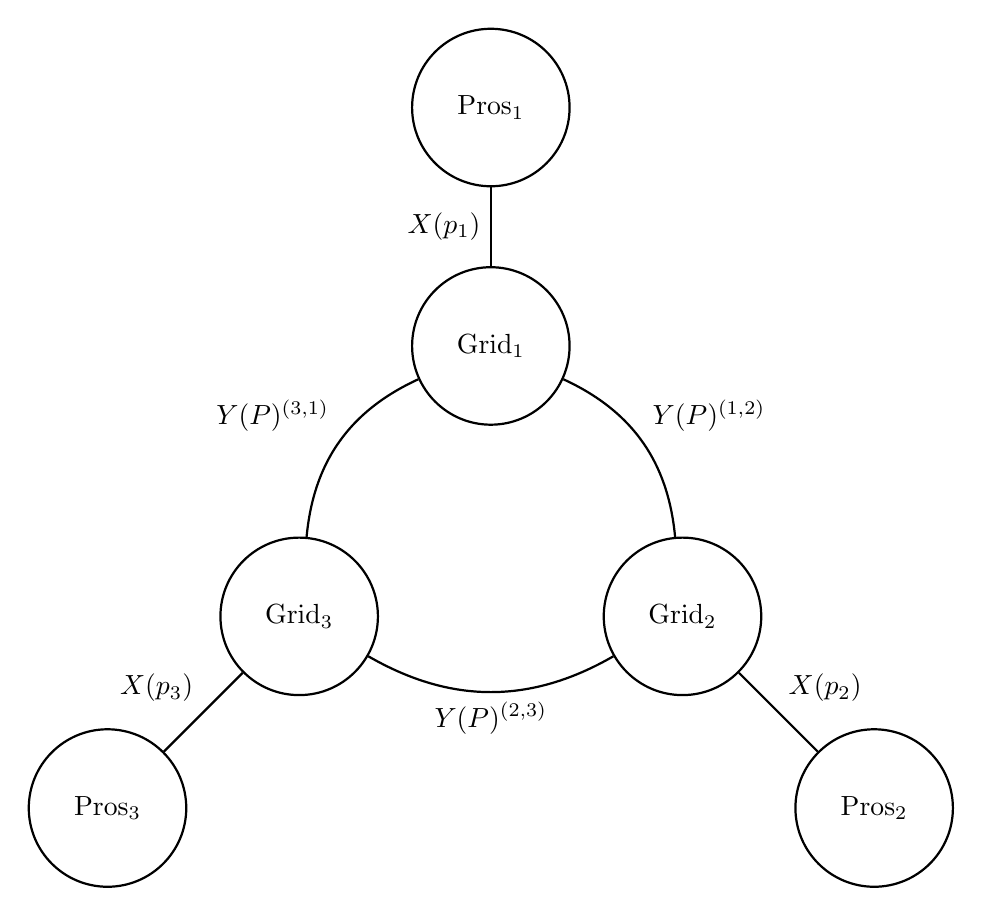
\begin{tikzpicture}[-, thick]
        % Grids
        \node[main node] (1) {Grid$_1$};
        \node[main node] [below right = 2cm and 1cm of 1] (2) {Grid$_2$};
        \node[main node] [below left = 2cm and 1cm of 1] (3) {Grid$_3$};
        % Local markets 
        \node[main node] [above = 1cm of 1] (5) {Pros$_1$};
        \node[main node] [below right = 1cm and 1cm of 2] (6) {Pros$_2$};
        \node[main node] [below left = 1cm and 1cm of 3] (7) {Pros$_3$};
        % Paths
        \path[draw,thick]
        (1) edge [bend left] node [above right] {$Y(P)^{(1, 2)}$} (2)
        (2) edge [bend left] node [below] {$Y(P)^{(2, 3)}$} (3)
        (3) edge [bend left] node [above left] {$Y(P)^{(3, 1)}$} (1)
        (1) edge node [left] {$X(p_{1})$} (5)
        (2) edge node [above right] {$X(p_{2})$} (6)
        (3) edge node [above left] {$X(p_{3})$} (7);
    \end{tikzpicture}
\end{center}

\section{Prosumers}

\subsection{Normal preferences}

The prosumer instantaneous utility of electricity consumption is,

\begin{equation*}
    u_i(x) = d_i \cdot \ln(x),
\end{equation*}

where $d_i$ is an heterogenous demand parameter.

Furthermore, agents get electricity endowment $e_{i, t}$ which follows a random exogenous process and have a given stock of cash-in-hand $m_t$, starting from $m_0$. Furthermore agents can buy or sell electricity $x_t$ at price $p_t$.

The dynamic optimization problem is then,

\begin{equation*}
    \begin{split}
        V(e_t) &= \sup_{x_t \in \R} \left\{u(x_t + e_t) + \beta \cdot \E_t V( e_{t+1} ) \right\} \\
        \\
        \textit{s.t. } m_{t+1} &= m_{t} - p_{t} \cdot x_{t}\\
        m_t  &\geq 0, \ m_0
    \end{split}
\end{equation*}

Hereafter we will suppress $i$ for convenience.

Agents are assumed to make forecasts over the price $p_{t+1}$, using a linear forecasting rule $\E_t[p_{t+1}] = \psi_h\cdot p_t$, where $\psi_h \in \Psi$ is selected in a manner similar to \citeauthor{Hommes2013} (\citeyear{Hommes2013}).

Using the budget constraint we can redefine the problem as,

\begin{equation}
    x_t = \frac{m_t - m_{t+1}}{p_t},
\end{equation}

such that the agents control variable is the next level of cash-in-hand $m_{t+1}$. This gives the Euler equation,

\begin{equation}
    u^\prime\left( e_t + \frac{m_t - m_{t+1}}{p_t} \right) = \beta \cdot \E_t \left[ u^\prime\left(e_{t+1} + \frac{m_{t+1} - m_{t+2}}{ \psi_h \cdot p_t} \right)  \right].
\end{equation}

The endogenous grid method can then be used to find a policy function

\begin{equation}
    m^\prime(m_t, p_t \ \vert \ \psi_h, e_t).
\end{equation}

The solution of the local problem yields the electricity demand in a state of high endowments and different conditions $m_t$ in Figure \ref{fig:demand} and the simulation run in Figure \ref{fig:sim}.

\begin{figure}[b]
    \centering
    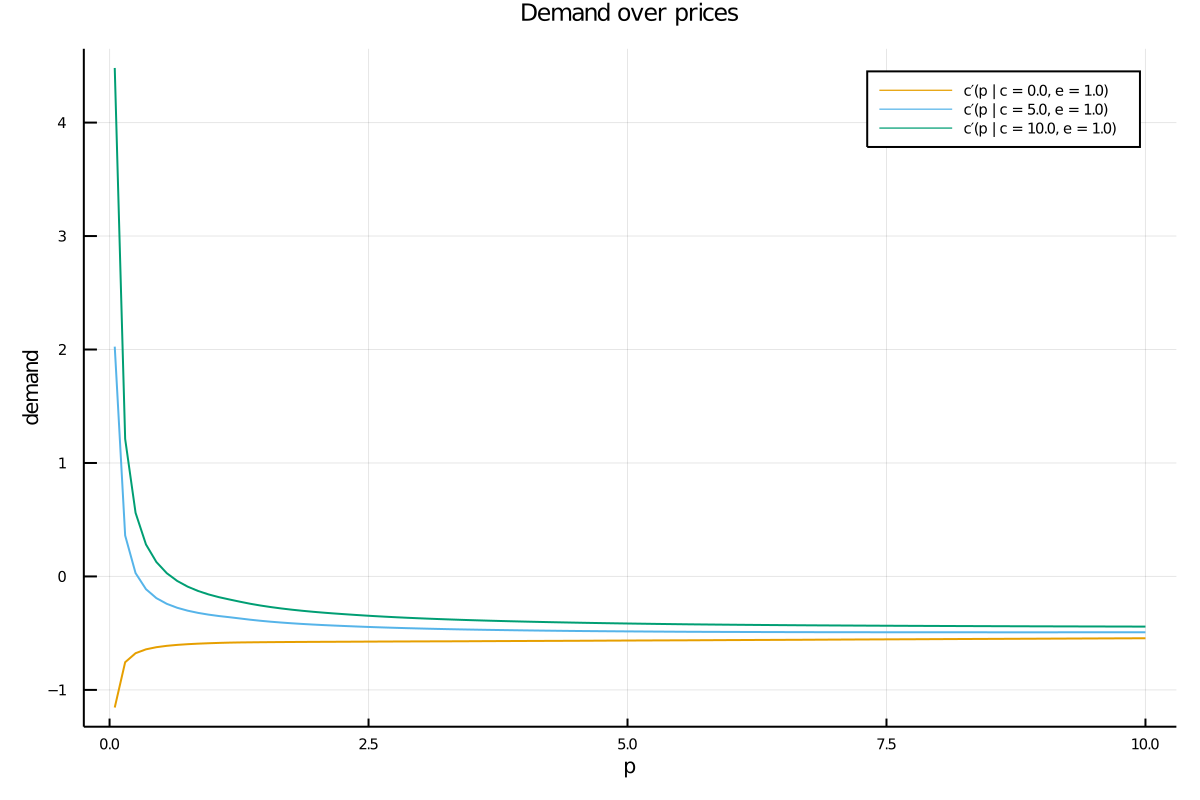
\includegraphics[width=0.9\textwidth]{../../plots/markets/pricedemand.png}
    \label{fig:demand}
    \caption{Electricity demand curve for an agent}
\end{figure}

\begin{figure}
    \centering
    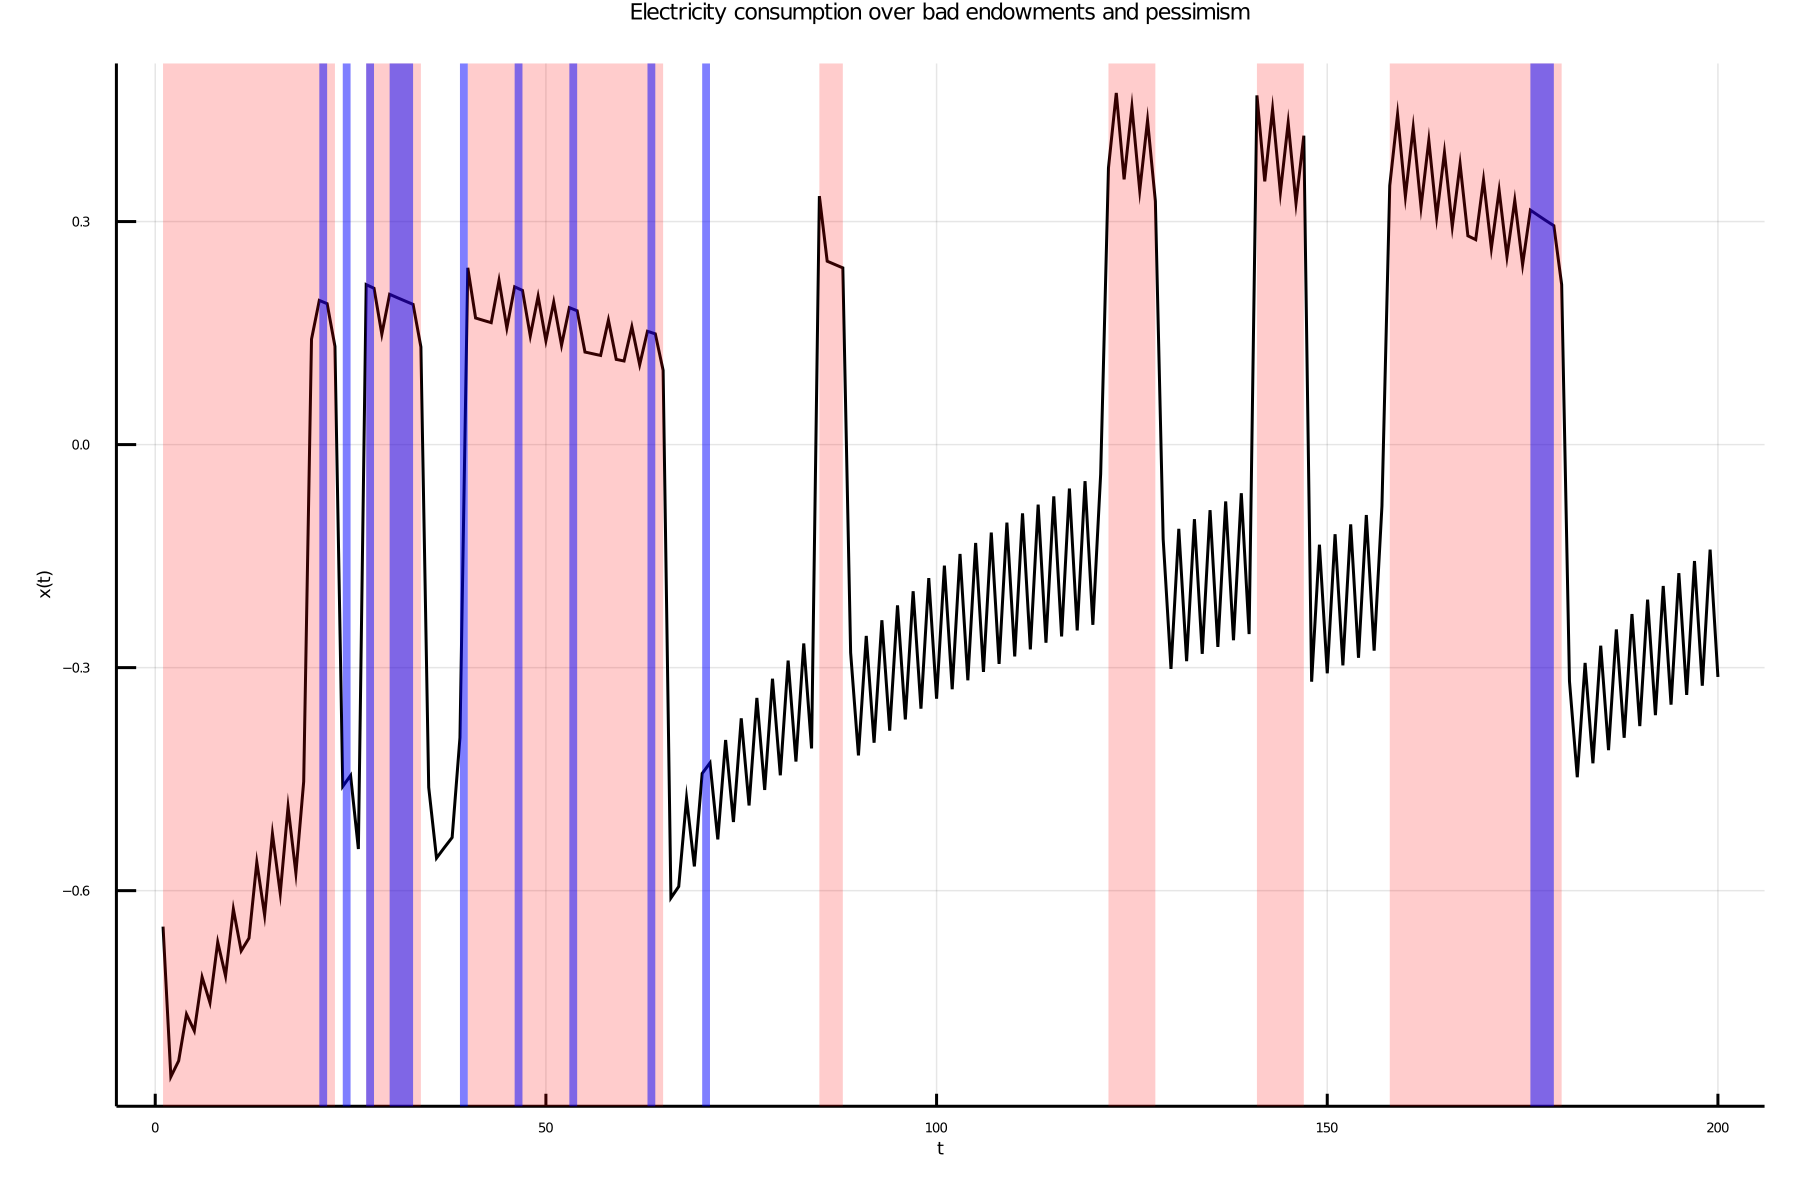
\includegraphics[width=0.9\textwidth]{../../plots/markets/simul.png}
    \label{fig:sim}
    \caption{Simulation of an agent with switching forecasting rule and $AR(1)$ price process}
\end{figure}

\begin{figure}
    \centering
    \includegraphics[width=0.9\textwidth]{../../plots/markets/kde.png}
    \label{fig:price}
    \caption{Prices in the above simulation}
\end{figure}

\iffalse
    \subsection{Epstein-Zin preferences}

    A better formulation, using Epstein-Zin preferences,

    \begin{equation}
        U_t = \left[ (1 - \beta) \cdot u(x_t)^{\frac{\phi - 1}{\phi}} + \beta \cdot \mu_t(U_{t+1})^{\frac{\phi - 1}{\phi}} \right]^{\frac{\phi}{\phi - 1}}
    \end{equation}

    where the certainty equivalent is,

    \begin{equation}
        \mu_t(U) = \E_t\left[ U^{1 - \gamma} \right]^{\frac{1}{1 - \gamma}}.
    \end{equation}

    As Caldara, introduce,

    \begin{equation}
        \theta := \frac{1 - \gamma}{1 - \frac{1}{\phi}}.
    \end{equation}

\fi

\section{Grid firms}

Grid firms face the optimization problem,

\begin{equation}
    \Pi^i\left(p^i_t, Y^{(i, j)}\right) = X^i_{t}(p^i_t) \cdot p^i_t - \sum_{j \in N(i)} Y^{(i, j)}_{t} \cdot P^{(i, j)}_t,
\end{equation}
subject to,
\begin{equation}
    X^i_t=  \sum_{j \in N(i)} Y^{(i, j)}_{t}
\end{equation}

For now assume $P_t^{(i, j)}$ is determined by (i.e. is a function of) the bargaining result $Y^{(i, j)}$.

The Lagrangian yields,

\begin{equation}
    \mathcal{L}\left(p, Y^j\right) = X(p) \cdot p - \sum_{j \in N(i)} Y_j \cdot P_j (Y_j) + \lambda\cdot \left(X(p) - \sum_{j \in N(i)} Y^j\right)
\end{equation}


\begin{equation}
    \begin{split}
        \frac{\partial}{\partial p} \mathcal{L} &= X^\prime(p) \cdot p + X(p) + \lambda \cdot X^\prime(p) = 0 \\
        \frac{\partial}{\partial Y^j} \mathcal{L} &= P_j + P^\prime_j \cdot Y_j + \lambda =0, \ \forall j \in N(i)
    \end{split}
\end{equation}

Isolating the multiplier $\lambda$ from the first equation yields,

\begin{equation}
    - \lambda = p + \frac{X}{X^\prime}(p)
\end{equation}

which yields the system of equations, $\forall j \in N(i)$,

\begin{equation}
    P_j(Y_j) + P^\prime_j(Y_j) \cdot Y_j = p + \frac{X}{X^\prime}(p)
\end{equation}

\newpage
\section{Bargaining model}

\subsection{Three firms}

Assume there are three, fully connected firms,

\begin{center}
    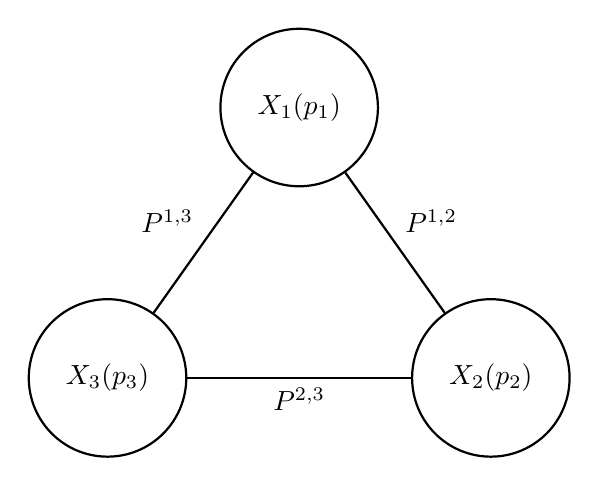
\begin{tikzpicture}[-, thick]
        % Grids
        \node[main node] (1) {$X_1(p_1)$};
        \node[main node] [below right = 2cm and 1cm of 1] (2) {$X_2(p_2)$};
        \node[main node] [below left = 2cm and 1cm of 1] (3) {$X_3(p_3)$};
        % Paths
        \path[-, draw,thick]
        (1) edge node [above right] {$P^{1, 2}$} (2)
        (2) edge node [below] {$P^{2, 3}$} (3)
        (1) edge node [above left] {$P^{1, 3}$} (3);
    \end{tikzpicture}
\end{center}

Firm's profits are,

\begin{equation}
    \begin{split}
        \Pi_1(P^{(1, 2)}, P^{(1, 3)}) &= X_1(p_1) \cdot p_1 - Y^{(1, 2)} \cdot P^{(1, 2)} - Y^{(1, 3)} \cdot P^{(1, 3)}\\
        \Pi_2(P^{(1, 2)}, P^{(2, 3)}) &= X_2(p_2) \cdot p_2 + Y^{(1, 2)} \cdot P^{(1, 2)} - Y^{(2, 3)} \cdot P^{(2, 3)} \\
        \Pi_3(P^{(1, 3)}, P^{(2, 3)}) &= X_3(p_3) \cdot p_3 + Y^{(1, 3)} \cdot P^{(1, 3)} + Y^{(2, 3)} \cdot P^{(2, 3)}
    \end{split}
\end{equation}

Note that $Y^{(1, 2)} > 0$ means that firm $1$ is buying from firm $2$.

The Nash bargaining solution is,

\begin{equation*}
    \begin{split}
        P^{(1, 2)} &= \arg \max_P \Pi_1(P, P^{(1, 3)}) \cdot \Pi_2(P, P^{(2, 3)} ) \\
        P^{(1, 3)} &= \arg \max_P \Pi_1(P^{(1, 2)}, P) \cdot \Pi_3(P, P^{(2, 3)} ) \\
        P^{(2, 3)} &= \arg \max_P \Pi_2(P^{(1, 2)}, P) \cdot \Pi_3(P^{(1, 3)}, P)
    \end{split}
\end{equation*}

The first order condition yields, $\Pi_1 = \Pi_2 = \Pi_3$

\subsection{General case}

Let $\matr{A} \in \R^{n\times n}$ be the adjacency matrix of the graph with associated lower triangular matrix $\matr{L_A}$. Let $\matr{G} = \matr{L_A} - \matr{L_A}^T$ with entries $g_{i, j} = -g_{j, i} \in \{-1, 0, 1\}$.

Then the payoff of node $i \in N = \{1, \ldots, n\}$ is,

\begin{equation}
    \Pi_i = X_i(p_i)\cdot p_i - \sum_{j \in N} g_{i, j} \cdot Y^{(i, j)} \cdot P^{(i, j)}
\end{equation}

Then,

\begin{equation}
    P^{(i, j)} = \arg \max_{P^{(i, j)}} \left\{\Pi_i \cdot \Pi_j \right\}
\end{equation}

with first order condition,

\begin{equation}
    \begin{split}
        \frac{\partial\Pi_i}{\partial P^{(i, j)}} \cdot \Pi_j &= - \frac{\partial\Pi_j}{\partial P^{(i, j)}} \cdot \Pi_i
    \end{split}
\end{equation}

which yields, forall $(i, j) : \ g_{i, j} \neq 0$,

\begin{equation}
    2\cdot P^{(i, j)} = X_i(p_i)\cdot p_i - X_j(p_j)\cdot p_j - \sum_{m \in N\setminus j} g_{i, m} \cdot Y^{(i, m)} \cdot P^{(i, m)} + \sum_{l\in N\setminus i} g_{j, l} \cdot Y^{(j, l)} \cdot P^{(j, l)}
\end{equation}

\iffalse % Weighted case

    \section{Weighted one prosumer case}

    Assume the local market has a one prosumers with type indicator $\mathbf{1}\{h_t = f\} = \eta_t$.

    \begin{equation}
        \begin{split}
            X_t(p) &= \eta_t \cdot x_{t, f} + (1 - \eta_t) \cdot x_{t, c} \\
            &= \eta_t \cdot \frac{m_t - g_f(m_t, p)}{p} + (1 - \eta_t) \cdot \frac{m_t - g_c(m_t, p)}{p}
        \end{split}
    \end{equation}


    Then,
    \begin{equation}
        \begin{split}
            \frac{\partial X}{\partial p} &= \frac{1}{p^2} \cdot \left[ \eta_t \cdot \left(\frac{\partial}{\partial p} g_f \cdot p + m_t - g_f \right) + (1 - \eta_t) \cdot \left(\frac{\partial}{\partial p} g_c \cdot p + m_t - g_c \right) \right] \\
            &=\frac{1}{p^2} \left[m_t + \eta_t \cdot \left( g^\prime_f \cdot p - g_f \right) + (1 - \eta_t) \cdot \left( g^\prime_c \cdot p - g_c \right) \right]
        \end{split}
    \end{equation}

    Hence,

    \begin{equation}
        \begin{split}
            \frac{X}{X^\prime} = p \cdot \frac{m_t - \eta_t \cdot g_f + (\eta_t - 1) \cdot g_c}{m_t + \eta_t \cdot ( g^\prime_f \cdot p - g_f ) + (1 - \eta_t) \cdot (g^\prime_c \cdot p - g_c)}
        \end{split}
    \end{equation}

    \begin{equation}
        \begin{split}
            \frac{X}{X^\prime} + p &= p \cdot \frac{m_t - \eta_t \cdot g_f + (\eta_t - 1) \cdot g_c}{m_t + \eta_t \cdot ( g^\prime_f \cdot p - g_f ) + (1 - \eta_t) \cdot (g^\prime_c \cdot p - g_c)} + 1 \\
            &= p \cdot  \frac{m_t - \eta_t \cdot g_f + (\eta_t - 1) \cdot g_c + m_t + \eta_t \cdot ( g^\prime_f \cdot p - g_f ) + (1 - \eta_t) \cdot (g^\prime_c \cdot p - g_c)}{m_t + \eta_t \cdot ( g^\prime_f \cdot p - g_f ) + (1 - \eta_t) \cdot (g^\prime_c \cdot p - g_c)} \\
            &= p \cdot \frac{2 \cdot m_t + \eta_t \cdot (g^\prime_f \cdot p - 2\cdot g_f) + (1 - \eta_t) \cdot (g^\prime_c \cdot p - 2\cdot g_c)}{m_t + \eta_t \cdot ( g^\prime_f \cdot p - g_f ) + (1 - \eta_t) \cdot (g^\prime_c \cdot p - g_c)}
        \end{split}
    \end{equation}

\fi

\iffalse % Case with discrete N
    Then,

    \begin{equation}
        \begin{split}
            X_t(p) &= \sum_{i\in f}  x_{t, i} + \sum_{j \in c} x_{t, j} \\
            &= \frac{\sum_{i \in f}  \left[m_{t, i} - g_f(m_{t, i}, p_t)\right]  + \sum_{j \in c}  \left[m_{t, j} - g_c(m_{t, j}, p_t)\right]}{p}
        \end{split}
    \end{equation}

    hence,

    \begin{equation}
        \begin{split}
            \frac{\partial}{\partial p} X_t(p) = &p \cdot \left[\sum_{i \in f} \frac{\partial}{\partial p} g_f + \sum_{j \in c} \frac{\partial}{\partial p} g_c  \right] + \\
            &+ \sum_{i \in f}  \left[m_{t, i} - g_f(m_{t, i}, p_t)\right]  + \sum_{j \in c}  \left[m_{t, j} - g_c(m_{t, j}, p_t)\right] = 0 \\
            0 &= \sum_{i \in f} \left[ m_{t, i} - g_f(m_{t, i}, p_t) + p \cdot \frac{\partial}{\partial p} g_f \right] + \sum_{j \in c}\left[m_{t, j} - g_c(m_{t, j}, p_t) +  p \cdot\frac{\partial}{\partial p} g_c\right]
        \end{split}
    \end{equation}

\fi

\end{document}